\documentclass{article}
\usepackage[utf8]{inputenc}
\usepackage{amsmath}
\usepackage{graphicx}
\usepackage{caption}
\usepackage{subcaption}

\title{Assignment 3}
\author{Juraj Šušnjara (s4846559)}
\date{November 2016}

\usepackage{natbib}
\usepackage{graphicx}

\begin{document}

\maketitle

\section{Exercise 1 – Bayesian linear regression}
\subsection{}

Data set consists of two data points:
\begin{equation}
    {x_1, t_1} = (0.4, 0.05)
\end{equation}
\begin{equation}
    {x_2, t_2} = (0.6, -0.35)
\end{equation}
Furthermore, we assume that $\alpha = 2$ and $\beta = 10$.

A target variable $t$ is linearly dependent on input variable $x$ subject to a random Gaussian noise with variance $\beta^{-1}$. Based on linear relationship we use regression model with polynomial basis functions of the form $f(x,\textbf{w}) = w_0 + w_1x$. For the weights, zero-mean Gaussian with precision $\alpha$ is assumed.

\begin{equation}
    t = a_0 + a_1x + \mathcal{N}(0, \beta^{-1})
\end{equation}
\begin{equation}
    \label{eq:basis}
    y(x,\textbf{w}) = \Phi(\textbf{x})^T\textbf{w} = w_0 + w_1x
\end{equation}
\begin{equation}
    p(\textbf{w}|\alpha) = \mathcal{N}(0, \alpha^{-1}\textbf{I})
\end{equation}
\begin{equation}
    p(t|x,\textbf{w},\beta) = \mathcal{N}(\Phi(\textbf{x})^T\textbf{w}, \beta^{-1})
\end{equation}

Relationship between prior, likelihood and posterior are shown in following equations:

\begin{equation}
    p(\textbf{w}|\alpha) = \mathcal{N}(0, \alpha^{-1}\textbf{I})
\end{equation}
\begin{equation}
    p(\textbf{t}|\textbf{w}, \textbf{x}) = \mathcal{N}(\textbf{t}|\Phi\textbf{w}, \beta^{-1}I)
\end{equation}
$$\Rightarrow$$
\begin{equation}
    p(\textbf{w}|\textbf{t},\textbf{x}) = \mathcal{N}(\textbf{w}|\textbf{m}_N, S_N)
\end{equation}
with
\begin{equation}
    \textbf{m}_N = \beta S_N \Phi^T\textbf{t}
\end{equation}
\begin{equation}
    S_N^{-1} = \alpha I + \beta \Phi^T\Phi
\end{equation}

Based on expression \ref{eq:basis} we can see that vector of basis functions is $\Phi(x) = \begin{pmatrix} 1 & x \end{pmatrix}^T$. Now we need to define and calculate $\Phi^Tt$ and $\Phi^T\Phi$ for our data set.

\begin{equation}
    \Phi^T\textbf{t} = \sum_n\Phi(x_n)t_n = N
    \begin{pmatrix}
        \mu_t \\
        \mu_{xt}
    \end{pmatrix}
\end{equation}
\begin{equation}
    \Phi^T\Phi = \sum_n\Phi(x_n)\Phi(x_n)^T = N
    \begin{pmatrix}
        1 & \mu_x \\
        \mu_x & \mu_{xx}
    \end{pmatrix}
\end{equation}

where

\begin{equation}
    \mu_t = \frac{1}{N} \sum_n t_n
\end{equation}
\begin{equation}
    \mu_x = \frac{1}{N} \sum_n x_n
\end{equation}
\begin{equation}
    \mu_{xt} = \frac{1}{N} \sum_n x_n t_n
\end{equation}
\begin{equation}
    \mu_{xx} = \frac{1}{N} \sum_n x_n^2
\end{equation}

We can use previous expressions in order to compute posterior:

\begin{equation}
    p(\textbf{w}|\textbf{t},\textbf{x}) = \mathcal{N}(\textbf{w}|\textbf{m}_N, S_N)
\end{equation}
\begin{equation}
    \textbf{m}_N = \beta S_N \Phi^T\textbf{t} = N \beta S_N 
    \begin{pmatrix}
        \mu_t \\
        \mu_{xt}
    \end{pmatrix}
\end{equation}
\begin{equation}
    S_N^{-1} = \alpha I + \beta \Phi^T\Phi = 
    \begin{pmatrix}
        \alpha & 0 \\
        0 & \alpha
    \end{pmatrix}
    + N \beta 
    \begin{pmatrix}
        1 & \mu_x \\
        \mu_x & \mu_{xx}
    \end{pmatrix}
\end{equation}

Predictive distribution is given by expression \ref{eq:pred} and it can be derived using the previously obtained posterior $p(\textbf{w}|\textbf{t},\textbf{x})$ as the prior for new observation and integrating out \textbf{w}.
\begin{equation}
    \label{eq:pred}
    p(t|x,\textbf{t},\textbf{x},\alpha,\beta) = \mathcal{N}(t|m(x),s^2(x))
\end{equation}

\begin{equation}
    p(\textbf{w}|\textbf{t},\textbf{x}) = \mathcal{N}(\textbf{w}|\textbf{m}_N, S_N)
\end{equation}
\begin{equation}
    p(t|\textbf{w},\textbf{t},\textbf{x}) = \mathcal{N}(t|\Phi(x)^T\textbf{w}, \beta^{-1})
\end{equation}
$$\Rightarrow$$
\begin{equation}
    p(t|x,\textbf{t},\textbf{x}) = \mathcal{N}(t|m_N^T\Phi(x), \sigma_N^2(x))
\end{equation}
where
\begin{equation}
    \sigma_N^2(x) = \frac{1}{\beta} + \Phi(x)^TS_N\Phi(x)
\end{equation}

Finally we can derive expressions for $m(x)$ and $s^2(x)$:
\begin{equation}
    m(x) = \Phi(x)^Tm_N = N\beta
    \begin{pmatrix}
        1 & x
    \end{pmatrix}
    S_N
    \begin{pmatrix}
        \mu_t \\ \mu_{xt}
    \end{pmatrix}
    = 
    \begin{pmatrix}
        1 & x
    \end{pmatrix}
    \begin{pmatrix}
        -0.0445 \\
        -0.2021
    \end{pmatrix}
\end{equation}

\begin{equation}
\begin{split}
    s^2(x) = \beta^{-1} \Phi(x)^T S_N \Phi(x) = \beta^{-1} +
    \begin{pmatrix}
        1 & x
    \end{pmatrix}
    S_N
    \begin{pmatrix}
        1 \\ x
    \end{pmatrix} \\
    = 0.1 +
    \begin{pmatrix}
        1 & x
    \end{pmatrix}
    \begin{pmatrix}
        0.1233 & -0.1712 \\
        -0.1712 & 0.3767
    \end{pmatrix}
    \begin{pmatrix}
        1 \\ x
    \end{pmatrix}
\end{split}
\end{equation}

\begin{equation}
    S_N^{-1} =
    \begin{pmatrix}
        \alpha & 0 \\
        0 & \alpha
    \end{pmatrix}
    + N \beta 
    \begin{pmatrix}
        1 & \mu_x \\
        \mu_x & \mu_{xx}
    \end{pmatrix}
\end{equation}

\subsection{}
The plot is shown in figure \ref{fig:meandev}. The figure clearly shows that currently, the initial prior still has a large effect. In a maximum likelihood solution, the line would now go through both of the data points. This can be shown by taking a lower value of $\alpha$ (or taking higher $\beta$), which will decrease the prior's certainty. The difference with the figure 3.8b in Bishop is explained by the fact that we use only a two-dimensional Gaussian basis function $\phi_j$, whereas Bishop uses 9.

\begin{figure}[htb]
\centering
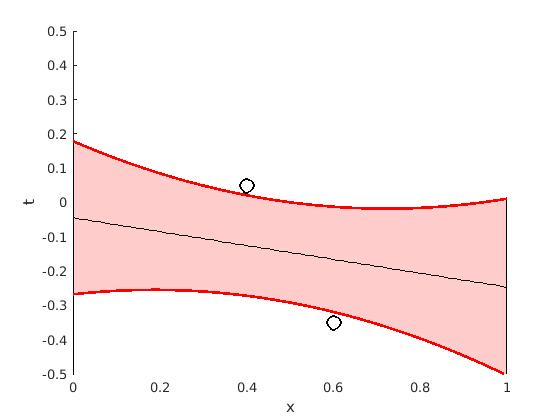
\includegraphics[width=10cm]{ex1_2.jpg}
\caption{Mean and deviation of predictive Gaussian distribution with 2 points that are our data set.}
\label{fig:meandev}
\end{figure}

\subsection{}

\begin{figure}[htb]
\centering
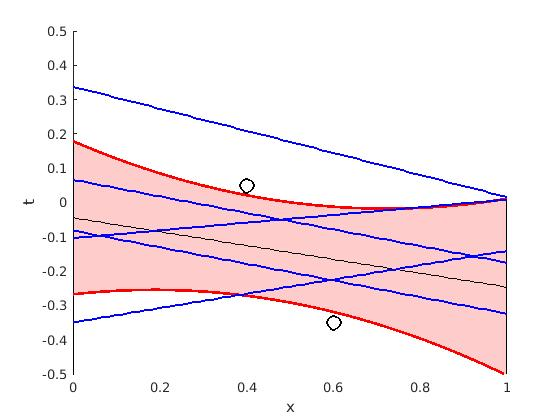
\includegraphics[width=10cm]{ex1_3.jpg}
\caption{Blue lines represent 5 different functions $y(x,\textbf{w})$ where weights are sampled from posterior distribution with mean $m_N$ and variance $S_N$}
\label{fig:pos}
\end{figure}

\end{document}
